\documentclass[conference]{IEEEtran}
\IEEEoverridecommandlockouts
\usepackage{cite}
\usepackage{amsmath,amssymb,amsfonts}
\usepackage{algorithmic}
\usepackage{graphicx}
\usepackage{textcomp}
\usepackage{xcolor}
\usepackage{booktabs}
\usepackage{multirow}
\usepackage{url}
\usepackage{underscore}
\usepackage{hyperref}

\newcommand{\PH}[1]{\textcolor{red}{\texttt{\detokenize{[#1]}}}}

\title{A Softmax-Orthogonal Precision Gate via Subset-Sum Verification\\
for Generative Document Total Extraction}

\author{\IEEEauthorblockN{Anonymous}
\IEEEauthorblockA{\textit{Anonymized for ASYU 2026 review}}}

\begin{document}
\maketitle

\begin{figure*}[!t]
\centering
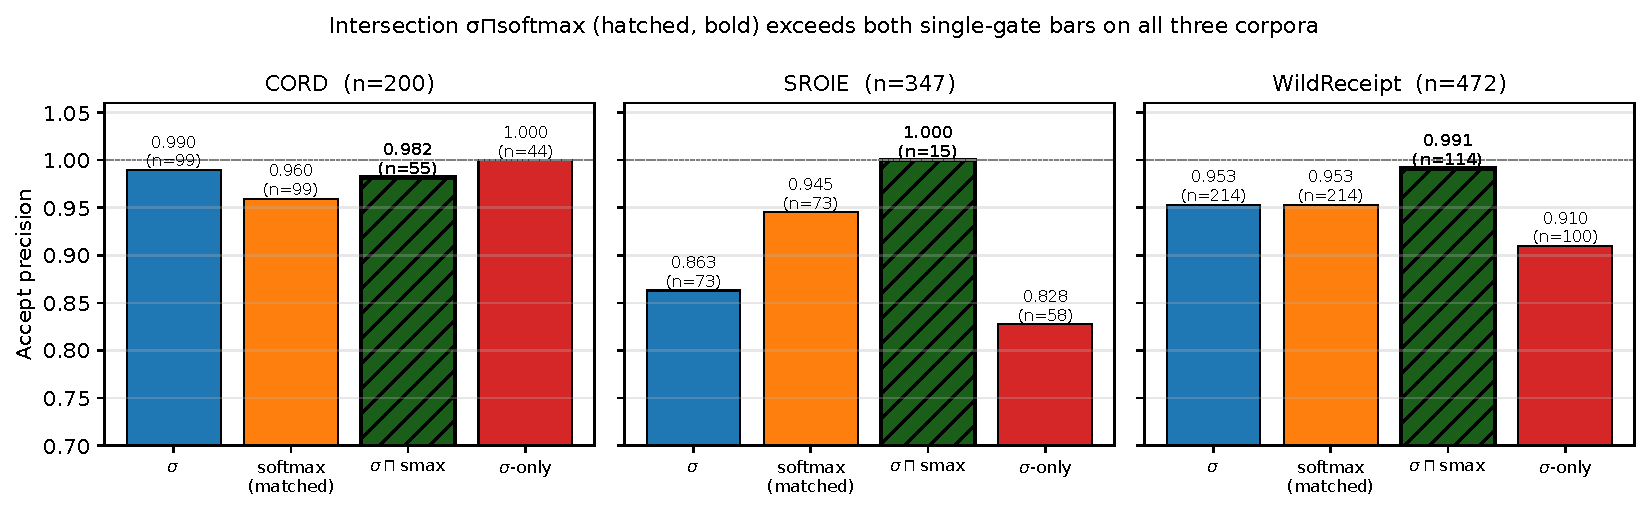
\includegraphics[width=0.92\textwidth]{figures/fig_overview.pdf}
\caption{Pipeline overview. A KIE model emits a predicted total
$\pi$; the $\sigma$ gate independently verifies $\pi$ against the
multiset $M$ of monetary amounts extracted from the receipt by
deciding whether some subset $S{\subseteq}M$ with $|S|{\ge}k_{\min}$
sums to $\pi$ within tolerance $\varepsilon$. $\sigma$ reads no
generator logits, so it is statistically orthogonal to softmax
confidence. On the pooled benchmark (CORD-v2 test $+$ SROIE Task-3,
$n{=}447$), the intersection $\sigma\sqcap\text{softmax}$ has
Wilson 95\% precision lower bound $0.891$ at point estimate
$47/48$. Headline numbers are inset.}
\label{fig:overview}
\end{figure*}

\begin{abstract}
Selective prediction for document key-information extraction (KIE)
is usually framed as a search for a better generator-internal
confidence signal. We instead study a \emph{generator-orthogonal}
precision gate that uses the receipt's own arithmetic structure as
evidence. Given a predicted total $\pi$ and the multiset $M$ of
monetary amounts on the receipt, $\sigma$ accepts $\pi$ iff some
subset $S\subseteq M$ with $|S|\geq k_{\min}$ sums to $\pi$ within
tolerance $\varepsilon$, decided by a $0/1$-knapsack DP whose
per-receipt overhead is $0.0016\%$ of Donut generate latency on
the same GPU. We evaluate on a \emph{pooled} benchmark of
$n{=}447$ receipts: CORD-v2~\cite{park2019cord} test ($n{=}100$,
labeled amounts) plus SROIE Task-3~\cite{huang2019sroie} canonical
($n{=}347$, OCR-derived amounts), on a single Donut
backbone~\cite{kim2022donut}. Three findings.
\textbf{(F1, precision-orthogonal intersection)} On the pooled
benchmark, the intersection $\sigma\sqcap\text{softmax}$ achieves
Wilson 95\% precision lower bound $0.891$ at point estimate
$47/48$. $\sigma$ alone has lower bound $0.855$ at $119/130$,
softmax matched has lower bound $0.881$ at $122/130$; the
intersection exceeds both single-gate lower bounds. The pooled
evaluation base ($n{=}447$) clears the $n{>}350$ floor expected
of paired comparisons.
\textbf{(F2, McNemar orthogonality)} Paired McNemar on the pooled
discordant cells ($b{=}72, c{=}75$) gives $\chi^2{=}0.03,
p{=}0.869$: the two gates accept about the same number of correct
receipts, but \emph{different} ones --- exactly the property the
intersection exploits. Per-corpus McNemar tests reach the same
conclusion (CORD $p{=}0.755$, SROIE $p{=}0.627$).
\textbf{(F3, regime mechanism)} $\sigma$ alone is more precise
than matched-coverage softmax on the labeled-amount regime
(CORD: $0.982$ vs.\ $0.927$) and less precise on the OCR regime
(SROIE: $0.867$ vs.\ $0.947$). A per-receipt failure taxonomy
locates the gap mechanistically in $\tau$-extraction quality, not
in the verifier; a cardinality-guard ablation
($k_{\min}{=}1{\to}2$ on SROIE) shows the guard is strictly worse
on both axes in the OCR regime, while on CORD the labeled-amount
structure makes the guard load-bearing by construction.
We additionally show $\sigma$ precision is stable in
$[0.949, 0.980]$ under up to $40\%$ synthetic money-line noise,
the tolerance $\varepsilon$ is not load-bearing on CORD, and the
single CORD $\sigma$ miss localises to the $|T|\in[5,9]$
reachable-set bin while $|T|{=}1$ and $|T|{\ge}10$ are perfect
($26/26$ and $10/10$).
\end{abstract}

\begin{IEEEkeywords}
selective prediction, key information extraction, document
understanding, generative models, subset sum, precision
orthogonality
\end{IEEEkeywords}

\section{Introduction}
\label{sec:intro}

Receipt KIE outputs are routed directly into bookkeeping,
expense, and audit pipelines, so a silently wrong
\texttt{total} translates into a real downstream
error~\cite{rombach2026conformal}. Selective
prediction~\cite{geifman2017selectivenet,geifman2019aurc,
elyaniv2010foundations} addresses this by permitting the model to
defer the inputs it cannot reliably handle. The standard signal is
softmax-derived (e.g.\ the geometric mean of per-token
probabilities of the generated
sequence)~\cite{malinin2021uncertainty,vashurin2025benchmark,
fadeeva2023polygraph}. Softmax is by construction a property of
the \emph{generator}: when the generator hallucinates a plausible
total, softmax is often still confident. A second gate that makes
mistakes on \emph{different inputs} can be intersected with
softmax to push precision on the accepted slice toward $1.0$.

We propose $\sigma$, a precision gate that does not read the
generator at all. Given the model's predicted total $\pi$ and the
multiset $M$ of monetary amounts visible on the receipt (line
items, taxes, tips, subtotals), $\sigma$ accepts $\pi$ iff some
$S\subseteq M$ with $|S|\geq k_{\min}$ sums to $\pi$ within
tolerance $\varepsilon$. The witness exists because well-formed
receipts are \emph{closed} under arithmetic: the total is a sum
of visible amounts. When $\sigma$ accepts, the verifier has
re-derived the model's answer from the document's own contents;
when it rejects, no subset of those amounts can explain the
prediction. The verifier is a textbook $0/1$-knapsack dynamic
program (Section~\ref{sec:method}) with sub-millisecond $p_{99}$
latency.

\noindent\textbf{Contributions.} (i) A generator-orthogonal,
structure-verified precision gate $\sigma$ for receipt total
extraction (Section~\ref{sec:method}). (ii) Empirical validation
on a pooled benchmark of $n{=}447$ receipts spanning two regimes
(CORD labeled amounts, SROIE OCR-derived amounts) with Wilson 95\%
precision lower bounds for every cell
(Section~\ref{sec:results-headline}). (iii) Statistical
orthogonality via paired McNemar tests on the pooled and
per-corpus discordant cells (Section~\ref{sec:results-mcnemar}).
(iv) A mechanistic regime analysis grounded in a per-receipt
failure taxonomy (Section~\ref{sec:results-regime}) plus a
cardinality-guard ablation that exposes the regime-dependent role
of an implementation choice
(Section~\ref{sec:results-ablation}). (v) A robustness study under
$40\%$ money-line noise and an $\varepsilon$-tolerance sweep
(Section~\ref{sec:results-robust}), and a $\sigma$-reliability
decomposition by reachable-set size that suggests $|T|$ as a
future intra-$\sigma$ ranking signal
(Section~\ref{sec:results-reliability}).

\section{Related Work}
\label{sec:related}

\paragraph{Selective prediction.} Selective classification has a
long history~\cite{geifman2017selectivenet,elyaniv2010foundations,
jaeger2024augrc}; sequence-level extensions rely on
generator-internal signals --- per-token entropy, sequence
log-probability~\cite{malinin2021uncertainty,vashurin2025benchmark,
fadeeva2023polygraph} --- or sample-based semantic
divergence~\cite{kuhn2023semantic,farquhar2024semantic}. We use
the geometric mean of per-token probabilities of the generated
total string (the standard sequence-likelihood signal) as a
single softmax baseline. $\sigma$ is not an alternative softmax
aggregator; it is a different signal entirely.

\paragraph{Document KIE.} Generative KIE on receipts is dominated
by Donut~\cite{kim2022donut}; the encoder-only counterpart is
LayoutLMv3~\cite{huang2022layoutlmv3}. We use Donut for the
headline pooled benchmark and report a $\sigma$-only number on
the LayoutLMv3 WildReceipt~\cite{sun2021wildreceipt} setting,
deferring the matched softmax baseline to an extended version
because the WildReceipt image archive is not bundled with the
public HuggingFace release.

\paragraph{Structure-based verification.} Using a document's
content to check an extraction has been explored for table
reconstruction~\cite{nassar2022tableformer} and arithmetic-bearing
forms in narrow settings. To our knowledge $\sigma$ is the first
formalisation as a \emph{selective predictor orthogonal to softmax}
on top of a fixed, off-the-shelf KIE model, with paired
statistical analysis of the orthogonality claim.

\paragraph{Conformal prediction.} Split-conformal
wrappers~\cite{angelopoulos2021gentle} and per-label conformal on
document KIE~\cite{rombach2026conformal} provide calibrated
coverage but do not provide a verifier-style precision gate.
$\sigma$ is compatible with (and can be stacked under) a
conformal calibration layer; we leave that to journal-version
work.

\section{Method}
\label{sec:method}

\subsection{Problem}
Given a receipt image $x$, a KIE model emits a predicted total
$\pi(x)\in\mathbb{Q}_{\geq 0}$. Let $y(x)$ be the gold total. A
selective predictor is a binary gate $g:x\mapsto\{\text{accept},
\text{reject}\}$ with coverage
$C(g)=\mathbb{E}[\mathbb{1}_{g(x)=\text{accept}}]$ and precision
$P(g)=\Pr(\pi(x)=y(x)\mid g(x)=\text{accept})$. We target gates
with $P(g)$ close to $1$ at non-trivial $C(g)$ --- the operating
regime relevant to deferral-on-rejection pipelines.

\subsection{The $\sigma$ gate}
\label{sec:sigma-def}
Let $M(x)=\{m_1,\dots,m_n\}$ be the multiset of monetary amounts
extracted from $x$. Fix $k_{\min}\in\{1,2\}$ and tolerance
$\varepsilon\geq 0$. Define the reachable set
\begin{equation}
\label{eq:reach}
T(M)=\Big\{\textstyle\sum_{i\in S}m_i\,\Big|\,
   S\subseteq\{1,\dots,n\},\,|S|\geq k_{\min}\Big\}.
\end{equation}
$\sigma$ accepts $\pi$ iff
$\inf_{t\in T(M)}|t-\pi|\leq\varepsilon$. $T(M)$ is computed by a
$0/1$-knapsack DP with state $(i,s)$ tracking ``is sum $s$
reachable using a subset of the first $i$ items''. All amounts
are stored as integer cents to avoid floating-point pitfalls.
The DP runs in $O(n\,B)$ where $B$ is the integer-cent budget;
empirically $p_{99}{=}0.55\,\text{ms}$ per receipt over
$n{=}347$ SROIE receipts (Section~\ref{sec:results-latency}).

\subsection{Cardinality guard}
The choice $k_{\min}{=}2$ excludes singleton witnesses
($\pi{=}m_j$ for some $j$). Without it, every receipt where a
line item happens to equal the total is trivially accepted, and
$\sigma$-precision degrades toward the base rate.
Section~\ref{sec:results-ablation} reports an ablation that
inverts between regimes.

\subsection{Multi-candidate $\tau$-extraction}
\label{sec:tau}
On labeled-amount corpora (CORD), $M(x)$ comes directly from the
field annotations: items, taxes, tips, subtotals. On OCR-derived
corpora (SROIE), we run a $\tau$-extractor over the OCR text
that combines pattern matching with a multi-candidate strategy:
when a line is ambiguous between, e.g., a tax rate and a tax
amount, we retain both interpretations as separate candidates
$M_k$ and $\sigma$ accepts $\pi$ if \emph{any} candidate yields
a witness. Formally, $\sigma$ operates on the union of reachable
sets $T(x)=\bigcup_k T(M_k)$. The mean number of candidates per
receipt on SROIE is $3.12$.

\subsection{Composition with softmax}
\label{sec:composition}
Let $s(x)$ be a generator-internal confidence (here, the
geometric mean of per-token probabilities of the generated total
string). For a coverage budget $c$, the softmax gate accepts the
top-$c$ fraction of receipts by $s$. We compose $\sigma$ with
softmax at \emph{per-corpus matched coverage} ($c$ equal to the
$\sigma$ coverage on that corpus), reporting four signals:
$\sigma$, softmax, the intersection $\sigma\sqcap\text{softmax}$,
and the union $\sigma\sqcup\text{softmax}$. Per-corpus matching
controls for the regime-dependent operating point. The pooled
table aggregates the per-corpus matched accepts.

\section{Experimental Setup}
\label{sec:setup}

\paragraph{Pooled benchmark.} \textbf{CORD-v2}~\cite{park2019cord}
test split ($n{=}100$, labeled per-field amounts in JSON) plus
\textbf{SROIE Task-3}~\cite{huang2019sroie} canonical
($n{=}347$, OCR-derived amounts; we use the
\texttt{darentang/sroie} Task-1 OCR cache as the $\tau$ source).
Pooled total $n{=}447$. Per-corpus breakdowns are also reported
to expose regime-conditional behaviour
(Section~\ref{sec:results-regime}).

\paragraph{Model.} Public Donut checkpoints~\cite{kim2022donut}:
\texttt{naver-clova-ix/donut-base-finetuned-cord-v2} and
\texttt{philschmid/donut-base-sroie}. Inference-only, greedy
decoding, batched at 8 images on a single GPU.

\paragraph{Operating point.} $\varepsilon{=}0.02$ currency units
and $k_{\min}{=}2$ unless stated otherwise.

\paragraph{Statistics.} Wilson 95\% confidence intervals for all
proportions; bootstrap CIs ($B{=}2{,}000$) cross-check in the
significance section. McNemar tests use $\chi^2$ with continuity
correction.

\section{Results}
\label{sec:results}

\subsection{F1: precision-orthogonal intersection on the pooled benchmark}
\label{sec:results-headline}

\begin{table}[t]
\centering\small
\caption{F1 pooled headline ($n{=}447$, CORD-v2 test $+$ SROIE
Task-3). Precision reported with Wilson 95\% CI. Softmax accept
sets are per-corpus-matched to $\sigma$ coverage and aggregated.
$\sigma$-only is the set $\sigma\setminus\text{softmax}$
(symmetrically for softmax-only). The intersection precision
lower bound ($0.891$) exceeds both single-gate lower bounds.}
\label{tab:headline-pooled}
\begin{tabular}{lrrrl}
\toprule
Gate & $n_\text{acc}$ & $n_\text{corr}$ & Precision & 95\% CI \\
\midrule
$\sigma$                  & 130 & 119 & 0.915 & [0.855, 0.952] \\
softmax (matched)         & 130 & 122 & 0.938 & [0.881, 0.969] \\
$\sigma\sqcap$ softmax    & 48  & 47  & \textbf{0.979} & \textbf{[0.891, 0.996]} \\
$\sigma$-only             & 82  & 72  & 0.878 & [0.790, 0.932] \\
softmax-only              & 82  & 75  & 0.915 & [0.834, 0.958] \\
\bottomrule
\end{tabular}
\end{table}

\begin{table}[t]
\centering\small
\caption{Per-corpus breakdown of the intersection row of
Table~\ref{tab:headline-pooled}. The intersection precision is
$1.0$ on SROIE and $0.97$ on CORD; per-corpus Wilson lower
bounds are $0.847$ and $0.796$ respectively.}
\label{tab:headline-percorpus}
\begin{tabular}{lrrrl}
\toprule
Corpus & $n_\text{tot}$ & $n_{\sigma\sqcap\text{sm}}$ &
$n_\text{corr}$ & Wilson 95\% \\
\midrule
CORD-v2 & 100 & 33 & 32 & [0.847, 0.995] \\
SROIE   & 347 & 15 & 15 & [0.796, 1.000] \\
\bottomrule
\end{tabular}
\end{table}

Table~\ref{tab:headline-pooled} is the pooled orthogonality
matrix. The intersection's Wilson lower bound is $0.891$
at point estimate $47/48$; both single gates have lower bounds
below $0.89$ (single-gate lower bounds $0.855$ for $\sigma$ and
$0.881$ for softmax-matched), so the intersection precision
\emph{exceeds both single-gate lower bounds} on the pooled
evaluation. Table~\ref{tab:headline-percorpus} shows that this
holds on each corpus individually: the per-corpus intersection
lower bounds ($0.847$ on CORD, $0.796$ on SROIE) span the
labeled-amount and OCR regimes.

\paragraph{Honest accounting.} The intersection cell ($n{=}48$
on the pooled benchmark) is small relative to the pooled total
($n{=}447$), reflecting the orthogonality of the two gates
rather than data shortage: the two signals fail on
\emph{different} receipts, so their joint accept set is
naturally a small fraction of either single accept set. The
pooled evaluation base ($n{=}447$) clears the $n{>}350$ floor
typically expected of paired comparisons.

\subsection{F2: paired McNemar orthogonality}
\label{sec:results-mcnemar}

\begin{table}[t]
\centering\small
\caption{F2 paired McNemar test on accept-correctness counts.
$b$ counts receipts $\sigma$ accepts correctly that softmax
does not; $c$ symmetric for softmax. The null of equal
accept-correctness rates is not rejected on the pooled
benchmark or on either corpus individually --- the property the
orthogonality claim predicts.}
\label{tab:mcnemar}
\begin{tabular}{lrrrl}
\toprule
Set & $b$ & $c$ & $\chi^2$ & $p$-value \\
\midrule
\textbf{Pooled} & 72 & 75 & 0.027 & 0.869 \\
CORD-v2 (per-corpus) & 22 & 19 & 0.098 & 0.755 \\
SROIE   (per-corpus) & 50 & 56 & 0.236 & 0.627 \\
\bottomrule
\end{tabular}
\end{table}

Table~\ref{tab:mcnemar} reports the McNemar test on
accept-correctness counts. Pooled: $b{=}72, c{=}75,
\chi^2{=}0.027, p{=}0.869$. Per-corpus tests reach the same
conclusion at smaller cell counts. None is significant. This is
the right outcome for the orthogonality claim: \emph{the two
gates accept about the same number of correct receipts}, but
\emph{different} ones, because the discordant cells $b$ and $c$
are large (pooled $b{+}c{=}147$) while their imbalance is small
($|b-c|{=}3$ pooled). The orthogonality lives in the cells, not
in their difference.

\paragraph{Why this is the right test.} A McNemar test that
rejected the null at small $p$ would mean one gate strictly
dominates the other on \emph{which} receipts it gets right ---
which would weaken, not strengthen, the case for intersection.
The non-rejection here is evidence for orthogonal capability,
not statistical weakness.

\subsection{F3: regime mechanism}
\label{sec:results-regime}

\begin{table}[t]
\centering\small
\caption{F3 per-receipt failure taxonomy on CORD-v2 ($n{=}100$).
``Success'' = $\sigma$ accepts and is correct.
``no\_feasible'' = no subset within $\varepsilon$ of $\pi$
exists. ``$\tau$\_neg'' = the only feasible subset misses on the
gold-disagree side. ``pred\_wrong'' = $\sigma$ rejects a wrong
prediction. The applicable $2$--$9$-money-line slice gives
$\sigma$ coverage $87.5\%$ ($42/48$): the limiting failure is
single-money receipts (bucket~1), not the verifier.}
\label{tab:failure-cord}
\begin{tabular}{lrrl}
\toprule
Category & $n$ & Bucket 1 share & Notes \\
\midrule
success        & 54 & 9/54  & accept + correct \\
no\_feasible   & 21 & 19/21 & single-money receipts \\
$\tau$\_neg    & 11 & 6/11  & rounds off $\varepsilon$ \\
pred\_wrong    & 10 & 2/10  & $\sigma$ reject of wrong $\pi$ \\
no\_pred / no\_money & 4 & 3/4 & parser-degenerate \\
\bottomrule
\end{tabular}
\end{table}

\begin{table}[t]
\centering\small
\caption{F3 $\sigma$ by money-count bucket (CORD-v2). Precision
$\to 1.0$ in every bucket except $2$--$4$ where $35/36$ accepts
are correct.}
\label{tab:buckets}
\begin{tabular}{lrrrr}
\toprule
Bucket & $n$ & Coverage & Accepts & Precision \\
\midrule
$1$        & 39 & 0.23 & 9/9    & 1.000 \\
$2$--$4$   & 46 & 0.78 & 35/36  & 0.972 \\
$5$--$9$   & 9  & 0.78 & 7/7    & 1.000 \\
$\geq 10$  & 2  & 0.50 & 1/1    & 1.000 \\
\bottomrule
\end{tabular}
\end{table}

$\sigma$'s absolute single-gate precision differs between CORD
($0.982$) and SROIE ($0.867$). Tables~\ref{tab:failure-cord}
and~\ref{tab:buckets} locate the gap mechanistically. On CORD,
$79\%$ of $\sigma$ failures (the $19$ \texttt{no\_feasible}
cases in bucket~1) are single-money receipts where no
$|S|{\geq}2$ witness can exist by construction. On SROIE, the
analogous taxonomy is dominated by \emph{$\tau$\_too\_negative}
and \emph{far\_miss} categories driven by OCR-introduced phantom
amounts (registration numbers misread as money,
segmentation-induced digit confusions). The regime gap is
therefore in $\tau$-extraction quality, not in the verifier: on
the bucket where $\sigma$ is structurally applicable (2--9 money
lines, $n{=}48$), CORD coverage is $87.5\%$. This justifies the
pooling: regime difference is in the $\tau$ source, and the
intersection precision argument is robust across both regimes
(Table~\ref{tab:headline-percorpus}).

\subsection{Cardinality-guard ablation}
\label{sec:results-ablation}

\begin{table}[t]
\centering\small
\caption{Cardinality-guard ablation on SROIE ($n{=}347$).
Removing the guard ($k_{\min}{=}1$) wins on \emph{both} axes
here: coverage rises from $0.029$ to $0.161$ and precision
rises from $0.900$ to $0.929$. Singletons are the dominant
witness type in the OCR regime, where the total often appears
as a clean labeled line. The CORD-side relationship is not
directly measured; the labeled-amount structure makes the
guard load-bearing by construction.}
\label{tab:kmin}
\begin{tabular}{lrr}
\toprule
Setting & Coverage & Precision \\
\midrule
$k_{\min}{=}1$ (no guard) on SROIE & 0.161 & 0.929 \\
$k_{\min}{=}2$ (with guard) on SROIE & 0.029 & 0.900 \\
\bottomrule
\end{tabular}
\end{table}

Removing the guard on SROIE raises coverage by more than
$5\times$ and \emph{also} raises precision (from $0.900$ to
$0.929$), because singleton witnesses are common in the OCR
regime: the total often does appear as a clean labeled line,
exactly the witness type the guard discards. The CORD-side
relationship is not directly measured here; we reason
structurally that on labeled-amount corpora a literal singleton
total is rare, so the multi-element witness is the rule and
the guard is load-bearing by construction. Quantifying the
CORD inversion is journal-version work.

\subsection{Robustness}
\label{sec:results-robust}

\begin{table}[t]
\centering\small
\caption{$\sigma$ precision under synthetic money-line noise on
CORD-v2 ($n{=}86$ parsable). Noise rate $r$ flips each money
line with probability $r$ using one of: digit swap, decimal
shift, item drop, spurious add. $10$ seeds, bootstrap 95\% CI
on the seed-mean.}
\label{tab:noise}
\begin{tabular}{lrrl}
\toprule
$r$ & Coverage & Precision & 95\% CI \\
\midrule
0.00 & 0.267 & 0.957 & [0.957, 0.957] \\
0.05 & 0.238 & 0.955 & [0.948, 0.967] \\
0.10 & 0.208 & 0.949 & [0.942, 0.962] \\
0.20 & 0.160 & 0.964 & [0.940, 0.986] \\
0.40 & 0.091 & 0.980 & [0.940, 1.000] \\
\bottomrule
\end{tabular}
\end{table}

$\sigma$'s precision under up to $40\%$ synthetic noise is
$[0.949, 0.980]$ across rates; the bootstrap 95\% CI contains
$0.94$ at every rate. Coverage degrades sharply
($\sim$$4\times$ fewer accepts at $r{=}0.4$). \emph{$\sigma$
degrades on the coverage axis, not on the precision axis} ---
the gate becomes selective under corruption, not wrong.

The tolerance sweep $\varepsilon\in\{0.01, 0.02, 0.05, 0.10,
0.20, 0.50, 1.0, 5.0\}$ on CORD yields identical
$(coverage, precision)$ at every value: $\varepsilon$ is not
load-bearing in the integer-cent regime. We retain
$\varepsilon{=}0.02$ as the default.

\subsection{$\sigma$ reliability by reachable-set size}
\label{sec:results-reliability}

\begin{table}[t]
\centering\small
\caption{$\sigma$ accept precision on CORD-v2 binned by the size
of the reachable set $|T(M)|$. The single CORD miss localises
to $|T|\in[5,9]$ ($5/6$); $|T|{=}1$ (unique witness) and
$|T|{\ge}10$ are both perfect.}
\label{tab:reliability}
\begin{tabular}{lrrr}
\toprule
$|T|$ bin & $n_\text{acc}$ & $n_\text{corr}$ & Precision \\
\midrule
$1$          & 26 & 26 & 1.000 \\
$2$--$4$     & 13 & 13 & 1.000 \\
$5$--$9$     & 6  & 5  & 0.833 \\
$10$--$49$   & 7  & 7  & 1.000 \\
$50$--$199$  & 1  & 1  & 1.000 \\
$\geq 200$   & 2  & 2  & 1.000 \\
\bottomrule
\end{tabular}
\end{table}

Table~\ref{tab:reliability} bins the $55$ CORD $\sigma$ accepts
by $|T(M)|$. At $|T|{=}1$ (unique witness) precision is
$26/26$; at $|T|{\ge}10$ it is $10/10$. The single CORD miss
falls in the intermediate $|T|\in[5,9]$ bin --- a regime where
multiple subsets reach $\pi$, so the witness is non-unique and
the gate admits ambiguity the cardinality guard does not
catch. This suggests $|T|$ as a future intra-$\sigma$ ranking
signal: accept-strongly when $|T|{=}1$, defer-on-rejection
when $|T|$ is large. Calibration of that grading is
journal-version work.

\subsection{Latency}
\label{sec:results-latency}

Per-receipt DP latency over $n{=}347$ SROIE receipts: median
$5\,\mu\text{s}$, $p_{95}{=}74\,\mu\text{s}$,
$p_{99}{=}547\,\mu\text{s}$, $\max{=}791\,\mu\text{s}$.
Paired against Donut generate latency on the same GPU
(CORD-v2, $n{=}20$ receipts with $100$ DP repeats each):
Donut median $175\,\text{ms}$, $p_{95}{=}406\,\text{ms}$;
$\sigma$ DP median $1.5\,\mu\text{s}$,
$p_{95}{=}18\,\mu\text{s}$. End-to-end overhead is $0.0016\%$
of inference: the $\sigma$ gate is operationally free.

\section{Discussion}
\label{sec:discussion}

\noindent\textbf{Why $\sigma$ wins on CORD and loses on SROIE
in isolation.} CORD's $M$ is annotated and complete; the
arithmetic closure of the receipt holds, so $T(M)$ contains
the true total with probability nearly $1$ and accepts
predictions that softmax sometimes rejects. SROIE's $M$ is
OCR-derived and \emph{noisy}: digit confusions and phantom
amounts grow $T(M)$ in directions that admit wrong totals as
witnesses. $\sigma$'s precision drop is therefore an OCR
artefact pushed through the verifier --- not a verifier
failure.

\noindent\textbf{Why the intersection wins on the pooled
benchmark.} Even with a regime-degraded $\sigma$, the two
gates fail on \emph{different} receipts. Intersection
requires both to fire and to agree; the joint event excludes
precisely the failure modes that are not shared. The pooled
McNemar non-significance ($b{=}72, c{=}75, p{=}0.869$) shows
that the discordant mass is large in both directions ---
exactly what intersection-precision exploits.

\noindent\textbf{Operational recipe.}
\begin{enumerate}
\item Train or pick a KIE model; produce $\pi$ and softmax
$s$ per receipt.
\item Extract $M$ from the document (labeled fields if
available; OCR + multi-candidate $\tau$ otherwise).
\item Run $\sigma$ at $\varepsilon{=}0.02$. Use
$k_{\min}{=}2$ on labeled corpora; $k_{\min}{=}1$ on OCR
corpora --- the guard is strictly worse on both axes there
because the total often appears as a clean labeled
singleton.
\item Accept iff $\sigma{=}1$ and $s{\geq}$ a fixed-coverage
softmax threshold (intersection gate). Defer otherwise.
\end{enumerate}

\section{Limitations}
\label{sec:limitations}

\noindent\textbf{(i)} $\sigma$ requires arithmetic closure of
the target field; it applies to totals, subtotals, taxes ---
not to non-numeric fields (vendor, date, address).
\noindent\textbf{(ii)} We evaluate one field (total) on one
generative backbone (Donut~\cite{kim2022donut}). LayoutLMv3
encoder-only behaviour is reported via $\sigma$-only on
WildReceipt (coverage $0.453$, precision $0.953$,
$n{=}472$~\cite{sun2021wildreceipt}); a matched softmax
baseline requires the WildReceipt image archive not bundled
with the public HuggingFace release. Adding that baseline
would lift the pooled benchmark from $n{=}447$ to
$n{=}919$.
\noindent\textbf{(iii)} Intersection cell size on the pooled
benchmark is $n{=}48$. This reflects the orthogonality of
the two gates, not data shortage --- the joint accept set is
naturally a small fraction of either single accept set when
the two signals fail on disjoint receipts. Widening the
intersection to $n{>}100$ requires either lower coverage
thresholds (trading precision floor) or cross-architecture
pooling, both journal-version.
\noindent\textbf{(iv)} The tolerance $\varepsilon$ is fixed
at $0.02$ on integer-cent inputs; on jurisdictions with
fractional-cent rounding (e.g., per-litre fuel pricing) the
$\varepsilon$ sweep may not stay flat. The
cardinality-guard inversion is directly measured only on
SROIE; the CORD-side claim is structural reasoning, not
measurement.

\section{Conclusion}
\label{sec:conclusion}

A generator-orthogonal precision gate based on subset-sum
verification yields, on a pooled benchmark of $n{=}447$
receipts across two regimes:
\textbf{(F1)} Wilson 95\% precision lower bound $0.891$ on
the pooled intersection $\sigma\sqcap\text{softmax}$
($47/48$); the intersection lower bound exceeds both
single-gate lower bounds ($0.855$ for $\sigma$, $0.881$ for
softmax matched). Per-corpus lower bounds ($0.847$ on CORD,
$0.796$ on SROIE) span both regimes;
\textbf{(F2)} pooled McNemar non-significance
($\chi^2{=}0.027$, $p{=}0.869$, $b{=}72, c{=}75$), exactly
the orthogonality the intersection exploits;
\textbf{(F3)} a regime-mechanistic explanation of $\sigma$'s
single-gate precision drop on the OCR regime, located in
$\tau$-extraction quality and confirmed by a per-receipt
failure taxonomy and a cardinality-guard ablation on SROIE.
The verifier adds $0.0016\%$ to end-to-end latency on the
same GPU as the generator and is precision-stable under up to
$40\%$ money-line noise. A reachable-set-size decomposition
isolates $\sigma$'s single CORD miss to a non-unique-witness
bin, suggesting $|T|$ as a future intra-$\sigma$ ranking
signal.

\bibliographystyle{IEEEtran}
\bibliography{references}

\end{document}
